\section{Setting Up Azure ML Python Development}\label{sec:PythonDevEnv}
\subsection{Understanding Python Kernel}
\subsubsection{Overview Python Interpreter}
Reference: \href{https://docs.python.org/3/tutorial/interpreter.html#the-interpreter-and-its-environment}{Using the Python Interpreter}, \href{https://blog.hubspot.com/website/what-is-python-interpreter#:~:text=A%20python%20interpreter%20is%20a,and%20low%2Dlevel%20languages%20are.}{What Is a Python Interpreter?}\\

\paragraph{High-Level Language}
The \gls{g_Python} language is a high-level programming language. This means, that the programming language is more similar to human language then to machine language, which is written in strings of bits - ones and zeros.
The advantage of it is that it is better understood by humans, but the same can not be said for the machines. Writing commands (instruction) in lines of zeros and ones is more difficult, that using higher level concepts. The gap between this, gets closes by the \textbf{Python Interpreter}.\\

The \gls{g_PyI} reads the command written by the \gls{g_Python} programmer, evaluates them, and returns the output. If the \textit{python.exe} application/ interpreter is opened, either through the \gls{CMD}, for example  
\begin{lstlisting}[style=CMD]
	$ python3.12
	\\\Python 3.12 (default, April 4 2022, 09:25:04)
	\\\[GCC 10.2.0] on linux
	\\\Type "help", "copyright", "credits" or "license" for more information.
	>>>
\end{lstlisting}
the commands
\begin{lstlisting}[style=CMD]
	>>> the_world_is_falt = True
	>>> if the_world_is_flat:
			print("Be careful not to fall off!")
	\\\ Be careful not to fall off!
\end{lstlisting}
or by opening the application directly.
\begin{figure}[H]
	\centering
	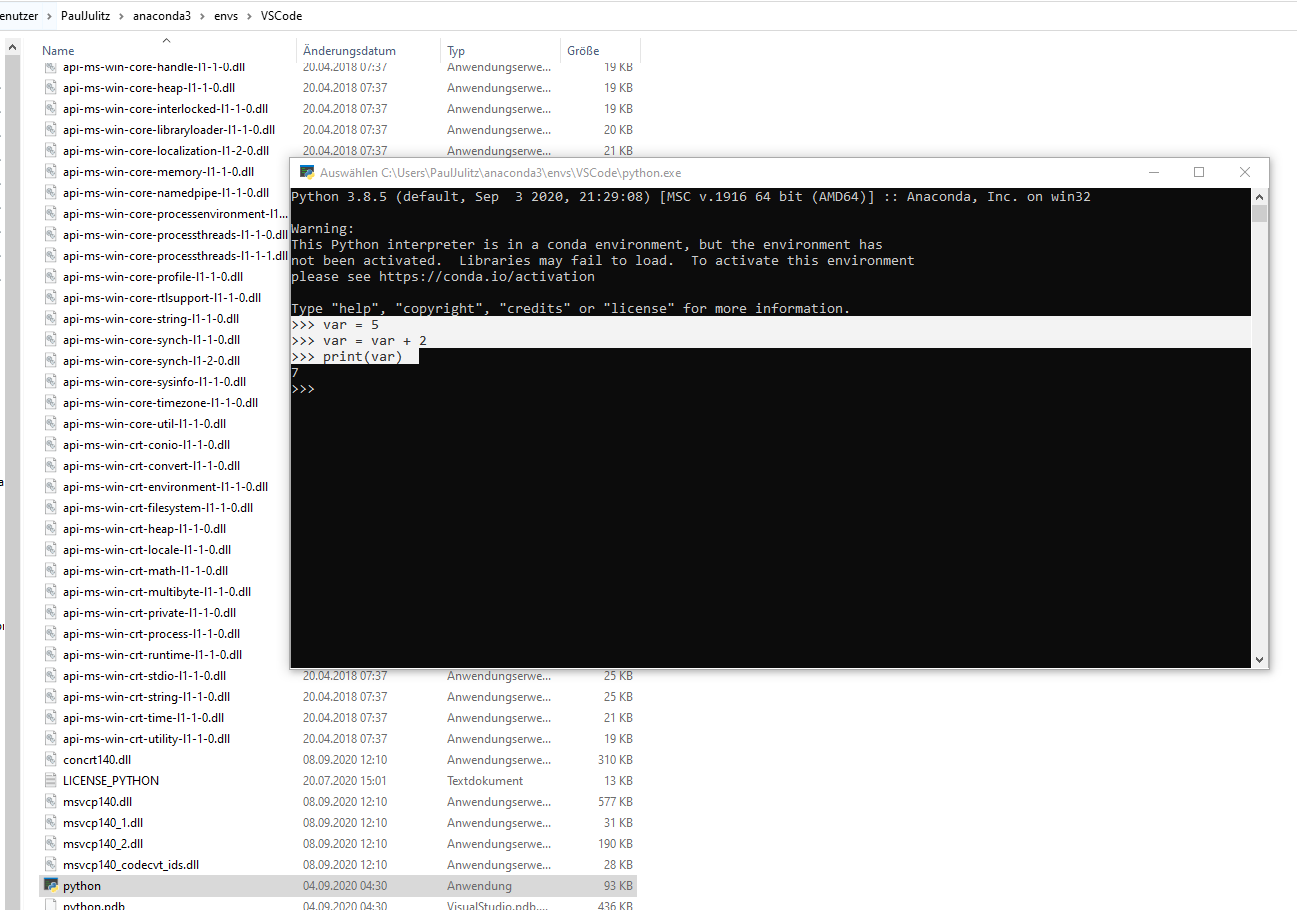
\includegraphics[scale = 0.2]{attachment/chapter_AML/Scc003}
	\caption{Using the command line with the python application/ interpreter}
\end{figure}
In both cases, the \gls{g_PyI} receives the commands and executes them. In the case where the \gls{IDE} is to write a the Python script (aka. module or application), the scripts gets passed to \gls{g_PyI}.\\

\paragraph{Difference between interpreter and a compiler}
Both the interpreter and compiler transforms the source code into binary machine code.
The difference arise through the way they are doing it differently: The interpreter translate the source code one statement at a time. The compiler on the other hand first scans the entire programm and then translate the whole program into machine code. For more detail, see \href{https://blog.hubspot.com/website/what-is-python-interpreter#:~:text=A%20python%20interpreter%20is%20a,and%20low%2Dlevel%20languages%20are.}{What Is a Python Interpreter?} or \href{https://www.analyticsvidhya.com/blog/2021/05/choose-best-python-compilers-for-your-machine-learning-project-detailed-overview/#:~:text=What%20is%20a%20Python%20compiler,executed%20directly%20by%20a%20computer.}{Best Python Compiler}
\begin{figure}[H]
	\centering
	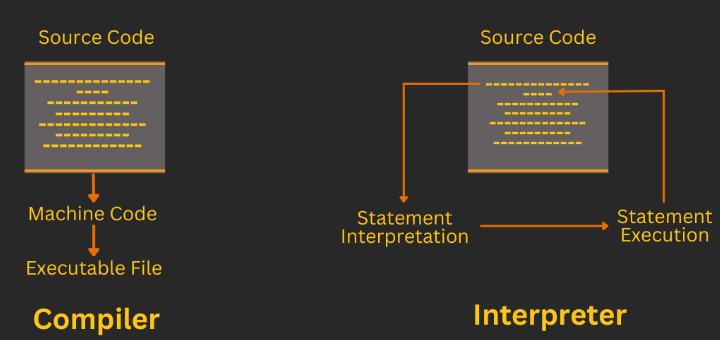
\includegraphics[scale = 0.3]{attachment/chapter_AML/Scc004}
	\caption{Example Compiler and Interpreter in Java}
\end{figure}

\subsubsection{ipykernel (Jupyter Notebook)}
Reference: \href{https://www.reddit.com/r/learnprogramming/comments/imhxai/what_is_the_difference_between_a_python_kernel_as/#:~:text=Python%20kernel%20is%20just%20a,is%20also%20not%20an%20interpreter.}{Difference Kernel and Interpreter}, \href{https://plotly.com/python/ipython-vs-python/}{IPython vs Python in Python}, \href{https://www.reddit.com/r/learnprogramming/comments/imhxai/what_is_the_difference_between_a_python_kernel_as/#:~:text=Python%20kernel%20is%20just%20a,is%20also%20not%20an%20interpreter.}{reddit:  difference between a Python Kernel (as in Jupyter notebooks) and a Python interpreter (like in PyCharm)?}, \href{https://python-forum.io/thread-40721.html}{jupyter kernel is an interface to the Python interpreter.} 
\\

\paragraph{IPython (Python3)}
To understand the \gls{g_Kernel_Jy_Py} it is helpful to understand \textit{IPython (Notebook)}. The \gls{g_PyI} passes command to it. This only allows commands for \gls{g_Python}.\\


\textit{IPyhton} creates an interactive command line terminal for \gls{g_Python}.  

\begin{figure}[H]
	\centering
	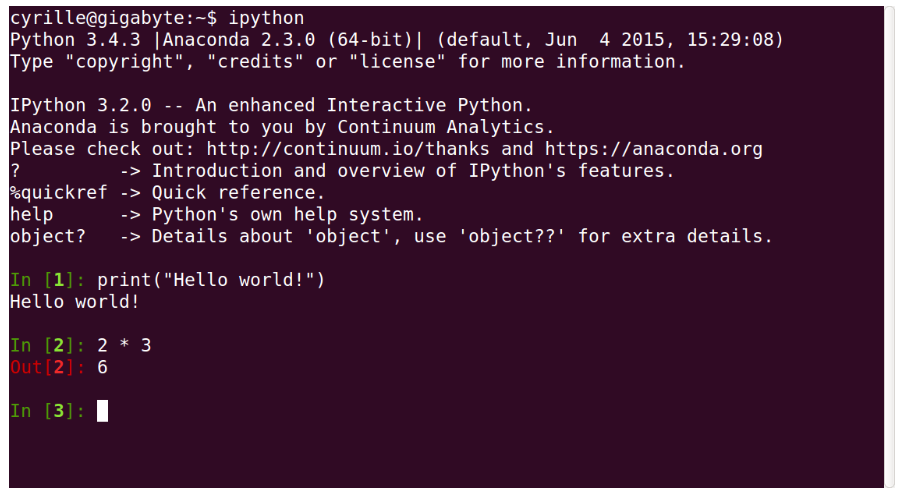
\includegraphics[scale = 0.3]{attachment/chapter_AML/Scc005}
	\caption{IPython interactive command-line terminal}
\end{figure}

\paragraph{Jupyter Notebook}
With the reorganization of \textit{IPython}, the new tool \textbf{Notebook} has been created. Under the project name \textbf{Jupyter}. This \gls{g_ipynb} is a web interface for \gls{g_Python}. It has the same interactive interface kept. Being a web-interface, it can integrate with many of the existing web libraries for data visualization.\\

The concept of a \textit{kernel} comes into play as the engine behind the web interface. The \textit{IPython} is now the backend with the \gls{g_Kernel_Jy_Py} for \gls{g_Python}. The \gls{g_Kernel_Jy_Py} with the advent of \gls{g_ipynb} is able to handel \textit{markdown} and \LaTeX text input.\\
\begin{figure}[H]
	\centering
	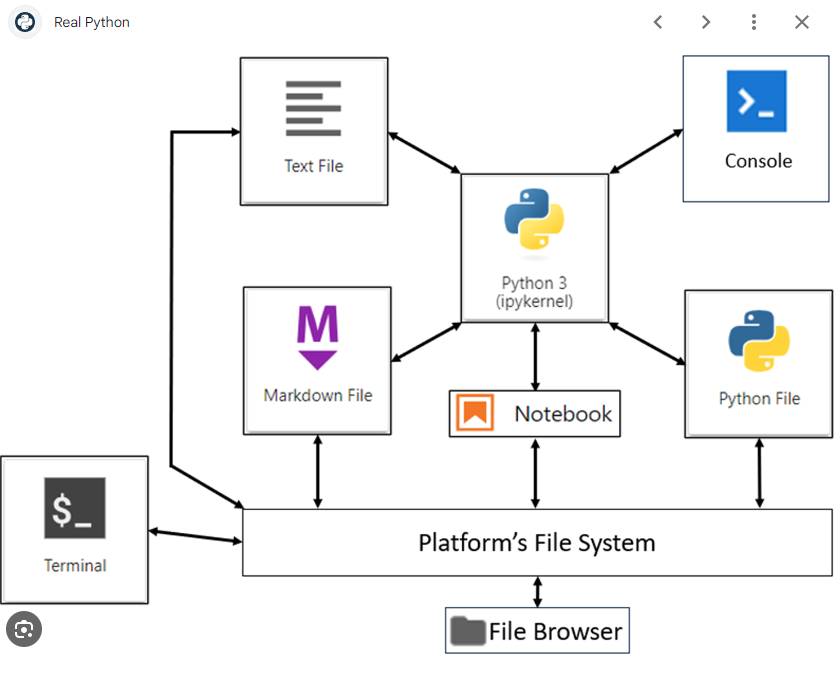
\includegraphics[scale = 0.3]{attachment/chapter_AML/Scc006}
	\caption{JupyterLab for an Enhanced Notebook}
\end{figure}
Note: The interaction with the \gls{g_Kernel_Jy_Py} is done through the \gls{g_ipynb}. With the latest tool: \textbf{Jupyter Lab}, interaction with separate files is possible.\\

$"$Inside$"$ the \gls{g_Kernel_Jy_Py} lives the \gls{g_PyI}. Another way of saying this is that the \gls{g_Kernel_Jy_Py} is the interface to the \gls{g_PyI}.

\subsubsection{Interacting with different (language) Kernels}
\paragraph{Theoretical Multi languages Kernel}
As said before the \gls{g_Kernel_Jy_Py} is for interacting with the \gls{g_PyI} and the other functionality of a \gls{g_ipynb}.\\

The community around, \textit{Juypter Notebook}, the application, developed more \gls{g_Kernel_Jy} for the \gls{g_ipynb}. Those \gls{g_Kernel_Jy} allows to interact with different languages like \textit{Ruby, Scale, R}.\\

It would be possible (Unclear how) to create a \gls{g_Kernel_Jy} which allows to interact with all those languages in one \gls{g_ipynb}. The current research for this chapter could not found one. For example the \gls{g_Kernel_Jy_Py} allows us to interact for example with \gls{g_Python}, Markdown, Shell Script. This does not conclude for example \gls{SQL}.

\paragraph{VSCode Compute Cells Confusion}
If a \gls{g_ipynb} is open, for each cell it is possible to select the language for this cell. This those two things. First it changes the \textit{IntelSence} syntax highlights. Secondly, it provides the \gls{g_Kernel_Jy} information about the lanuage which is used in this cell.

\begin{figure}[H]
	\centering
	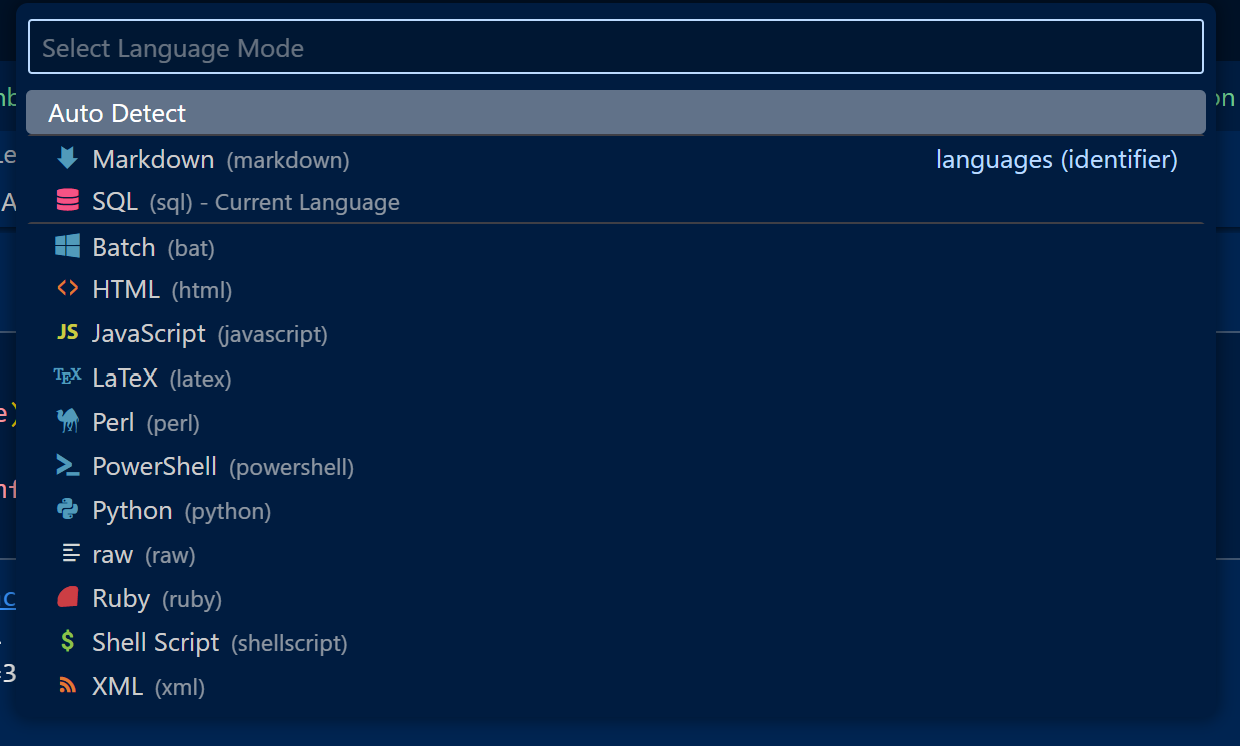
\includegraphics[scale = 0.3]{attachment/chapter_AML/Scc007}
	\caption{Cell Language Mode selection.}
\end{figure}

However, this \underline{does not mean} that all languages are supported by the selected \gls{g_Kernel_Jy}. 

\subsubsection{VEN and ipykernel}
% Spun up by Jupyter 
% Spn up on your machine
Starting with a \gls{g_ipynb}. In \gls{VEN} gets created either if a local server gets spin up or a Jupyter hosted server. Note: The a local server mean, the the web-interface get installed on you own machine. The compute resources are the onces from the own machine.

% Scc008

\begin{comment}
\subsubsection{Ipykernel (Notebook Style)}


%%  VENV and ipykernel
%%% What get's installed
%%%% IPython, ipython kernel, jupter notebook, python (interpreter) version etc.
%%%% Note: If the VENV get "spin" up for you, those objects get installed for this directory: Depending on the flexeblilty, there venv can be customizeable or not. Default Assumtion: Wenn a local Jupter notebook server gets spinn up, the python version 3 probablly with the neweset version get's installed.
%%%% Link to how to change python version in VENV in ipykernel.
%%%% Multiple kernels in once VENV. In contracst to the previous section. It is different, to install multiple kernels in once venv
%%%% lstlisting
%%%% command: jupyter kernelspec list ->
%%%% PS C:\Users\PaulJulitz\iCloudDrive\TexMaker\GitHub_Notizen_DSci\Notizen_DSci> jupyter kernelspec list
%%%% Available kernels:
%%%% python3    C:\Users\PaulJulitz\anaconda3\envs\Jupter\share\jupyter\kernels\python3
%%%% However, this can be installed, for each notebook can only be one kernel be activated.



%% Jupter Server
%%% Local and actually Jupyter Server



\subsection{IPython (Jupyter Notebook)}
%%% Umgang mit 

%% Maybe I start for now

%-Short: Juypter Notebook: Web Interface (Local host); Reference to Cloud Computing
%-
\paragraph*{Jupyter Notebook}
\paragraph*{VSCode, Synapse Notebooks}
% Kernel, SQL, Pyspark, SQLspark kernel

\paragraph*{Kernel}
\paragraph*{VSCode and Jupyter Notebook}
% - Web Interactive Interface
\paragraph*{Setting up VEnv}
\paragraph*{Jupyter Lab}
\subsection{Azure ML Extension (VSCode)}
\paragraph*{Configuration Workspace}
Or maybe in reference to the Kernel section
\subsection{Cloud-based Workstation (Compute Instance)}
 %-
% Setting up the Repo: VM enviroment
% Setting up a python development environment
% Environment
%% Local env
%% DSVM

% Okay, setting up Azure ML Python Develop environment
%% - Repo
%% - Learn Web interface
%-------------- I can do, what ever I'm able to to.
% Understanding Python Kernel
	Inhalt...
\end{comment}
